\documentclass{article}


% if you need to pass options to natbib, use, e.g.:
%     \PassOptionsToPackage{numbers, compress}{natbib}
% before loading neurips_2023


% ready for submission
\usepackage[final]{neurips_2023}
\usepackage{amsmath}
\usepackage{graphicx}
%\usepackage{subcaption}
\usepackage{subfig}

% to compile a preprint version, e.g., for submission to arXiv, add add the
% [preprint] option:
%     \usepackage[preprint]{neurips_2023}


% to compile a camera-ready version, add the [final] option, e.g.:
%     \usepackage[final]{neurips_2023}


% to avoid loading the natbib package, add option nonatbib:
%    \usepackage[nonatbib]{neurips_2023}


\usepackage[utf8]{inputenc} % allow utf-8 input
\usepackage[T1]{fontenc}    % use 8-bit T1 fonts
\usepackage{hyperref}       % hyperlinks
\usepackage{url}            % simple URL typesetting
\usepackage{booktabs}       % professional-quality tables
\usepackage{amsfonts}       % blackboard math symbols
\usepackage{nicefrac}       % compact symbols for 1/2, etc.
\usepackage{microtype}      % microtypography
\usepackage{xcolor}         % colors


\title{Dynamic Daylight Simulation with Snow Effect}

% The \author macro works with any number of authors. There are two commands
% used to separate the names and addresses of multiple authors: \And and \AND.
%
% Using \And between authors leaves it to LaTeX to determine where to break the
% lines. Using \AND forces a line break at that point. So, if LaTeX puts 3 of 4
% authors names on the first line, and the last on the second line, try using
% \AND instead of \And before the third author name.


\author{%
  Steven Webb\\\\
  u7544998 
   \And
  Mike Blue\\\\
  u333333\\
  \AND  The Australian National University 
}


\begin{document}


\maketitle


\begin{abstract}
  In order to preserve structural edges and shapes while simplifying the triangle mesh of man-made 3D models, we propose a new quadric error metric based on the distances between the new vertex position and the affected edges for edge collapse operations. With a 2D view sampling method, the contour and silhouette likelihood of the edges are computed, which act as the quadric’s weights during the mesh decimation. The comparisons and analysis among our methods with different weighting schemes will be presented in this report. We also compare our method with QSlim  and structure-aware mesh decimation method in multiple cases. Output generated by our method is better than QSlim and comparable to structure-aware method in most of the cases. 
\end{abstract}


\section{Introduction}

For our final project, we implemented a system for rendering forests of trees in real time. We are using the method outlined in Eric Bruneton and Fabrice Neyret’s Real-time Realistic Rendering and Lighting of Forests[1], specifically their z-field method for rendering trees of apparent sizes larger than a few pixels. Trees are often difficult to render in real-time applications as their geometry is complex, though simplified methods are easy to identify as lower quality. Our program provides fast and accurate rendering of trees as well as a fractal based landscape to simulate a forest. In this paper, we explain the motivation for this model, then describe the algorithms used. We finish up with some ideas for future work and some of the bugs we encountered.

Please read the instructions below carefully and follow them faithfully. 


\section{Motivation and Problem Statement}

Trees are often a plentiful part of landscapes, and so rendering them at the same level of fidelity as foreground objects can make real-time rendering impossible. At the same time, lower fidelity objects can detract from a scene’s appearance, even if they are part of the background.
 1
Moderate quality tree models can be 250,000 or more triangles[2]. Just 20 of such trees would involve 5 million polygons. For comparison, a frame in the 2007 game Lost Planet can have 3 million polygons in a frame. Clearly, conventional rendering methods do not permit the use of such tree models in games. Games must instead rely on include low quality tree models or other workarounds of reduced fidelity.
Bruneton and Fabrice [1] implemented a fast means of rendering high quality mid-distance trees, display- ing 180,000 such trees at over 30 frames per second. We hoped to duplicate their success, rendering tens of thousands of trees across a landscape in real time.
Papers to be submitted to NeurIPS 2023 must be prepared according to the
instructions presented here. Papers may only be up to {\bf nine} pages long,
including figures. Additional pages \emph{containing only acknowledgments and
references} are allowed. Papers that exceed the page limit will not be
reviewed, or in any other way considered for presentation at the conference.


The margins in 2023 are the same as those in previous years.


Authors are required to use the NeurIPS \LaTeX{} style files obtainable at the
NeurIPS website as indicated below. Please make sure you use the current files
and not previous versions. Tweaking the style files may be grounds for
rejection.


\section{Previous Works}
The ground under the trees is dynamically generated at runtime when the program is run. The diamond- square method of fractal terrain generation is used to create a height map, which is then applied to a square grid to create varied terrain. Points are set to the average height of particular surrounding points, then a random offset is added for variation. The offset is generated uniformly at random on the range (−x, x), where x is set before the algorithm is run, and is reduced by 2−y each iteration, where y can be adjusted. x is directly related to the maximum and minimum heights produced, and y is inversely related to the steepness of generated terrain. Lengths in the algorithm are the number of points between the current point and the other point in consideration, and can only be considered in horizontal or vertical lines. Points which are adjacent form a line of length zero. The diamond-square method in pseudocode [3] follows. 



The formatting instructions contained in these style files are summarized in
Sections \ref{gen_inst}, \ref{headings}, and \ref{others} below.


% \section{Our Method}
% \label{gen_inst}
% 
% 
% The text must be confined within a rectangle 5.5~inches (33~picas) wide and
% 9~inches (54~picas) long. The left margin is 1.5~inch (9~picas).  Use 10~point
% type with a vertical spacing (leading) of 11~points.  Times New Roman is the
% preferred typeface throughout, and will be selected for you by default.
% Paragraphs are separated by \nicefrac{1}{2}~line space (5.5 points), with no
% indentation.
% 
% 
% The paper title should be 17~point, initial caps/lower case, bold, centered
% between two horizontal rules. The top rule should be 4~points thick and the
% bottom rule should be 1~point thick. Allow \nicefrac{1}{4}~inch space above and
% below the title to rules. All pages should start at 1~inch (6~picas) from the
% top of the page.
% 
% 
% For the final version, authors' names are set in boldface, and each name is
% centered above the corresponding address. The lead author's name is to be listed
% first (left-most), and the co-authors' names (if different address) are set to
% follow. If there is only one co-author, list both author and co-author side by
% side.
% \subsection{ Displaying Trees}
% 
% For each tree in the forest, a quad is displayed and rotated around its center to face the camera. The view of the tree which is nearest to the angle between the tree and the camera is drawn to the quad. There is noticeable popping between the views since no interpolation is used, but with 300 views the transitions are smooth. Selection of the nearest view can be accomplished with simple arithmetic using the grid-like distribution of camera positions, while quad placement requires two vector cross products and some vector addition. These are some of the only computations that need to be done with each frame, allowing for interactive control of scenes of thousands of trees.
% 
% 
% 
% Please pay special attention to the instructions in Section \ref{others}
% regarding figures, tables, acknowledgments, and references.
% 

\section {Methods and Algorithms}
 
 
\subsection {Snow Rendering}
TODO: Snow Rendering and CG algorithms
\subsubsection {Snow Accumulation Prediction Function}



\begin{figure}[h]
  \centering
  \begin{minipage}{0.45\textwidth}
      \centering
      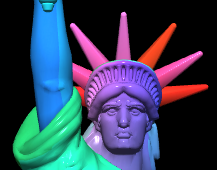
\includegraphics[width=\textwidth]{images/HeadManualWithoutSnow.png}
      \caption{First image caption}
      \label{fig:image1}
  \end{minipage}\hfill
  \begin{minipage}{0.45\textwidth}
      \centering
      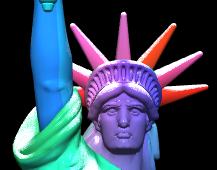
\includegraphics[width=\textwidth]{images/HeadManualWithSnow.png}
      \caption{Second image caption}
      \label{fig:image2}
  \end{minipage}
\end{figure}


\subsubsection {Snow Color Function}

\subsubsection {Full Snow Equation}

\subsection {Environment Simulation}

%  Environment 1: Temperature
\subsubsection {Temperature}
The temperature of a location depends on multiple factors, e.g., time of the day, season, altitude, 
latitude and distance to the ocean. To create a reasonable snow effect, the location used in this paper 
is an in-land city around the latitude of 35$^{\circ}$ N or 35$^{\circ}$ S and the season is winter.

This location has a large temperature difference. The highest temperature is about 
\(10^\circ\mathrm{C}\), which can be reached at around 1-2 P.M. The lowest temperature is about 
\(-10^\circ\mathrm{C}\), which can be reached at around 5-7 A.M. The hourly temperature data can be
obtained on weather forecast websites, and the Cubic Spline method is used to interpolate the 
intermediate values, making the temperature-time curve smoother.

%  Environment 2: Snow Amount
\subsubsection {Snow Amount}
The snow amount on an object is based solely on the environmental temperature. 
The range of it between 0 and 1, where 0 means that no snow on the object and 1 means
that the object is fully covered by snow.

If the temperature is below or equal to \(0^\circ\mathrm{C}\), the snow amount is always 1. 
If the temperature is above or equal to \(5^\circ\mathrm{C}\), the snow amount is always 0. 
Otherwise, the snow amount decreases linearly from 1 to 0 as temperature increases.

\[
  S=
  \left\{
    \begin{array}{ll}
      0 & t\leq 0 \\
      1 - \frac{t}{5} &  0 < t < 5 \\
      1 & t\geq 5 \\
    \end{array} 
  \right. 
\]
\text{where } t \text{ is the temperature in degrees Celsius.}

% The following figures are temperature - time relationship and snow amount - time relationship

\begin{figure}[h]
  \centering
  \begin{minipage}{0.45\textwidth}
      \centering
      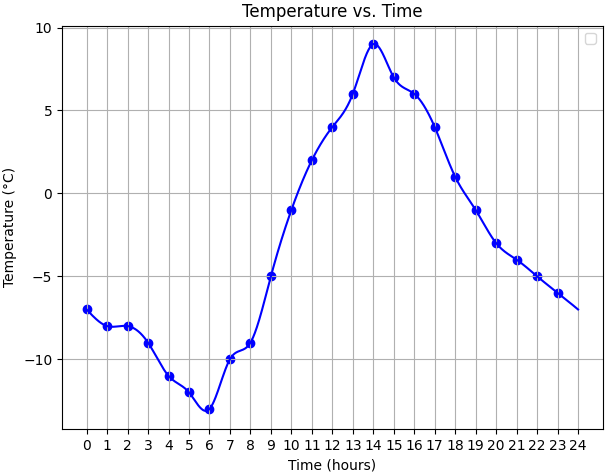
\includegraphics[width=\textwidth]{images/Temperature35N.png}
      \caption{Temperature throughout the day}
      \label{fig:Temperature35N}
  \end{minipage}\hfill
  \begin{minipage}{0.45\textwidth}
      \centering
      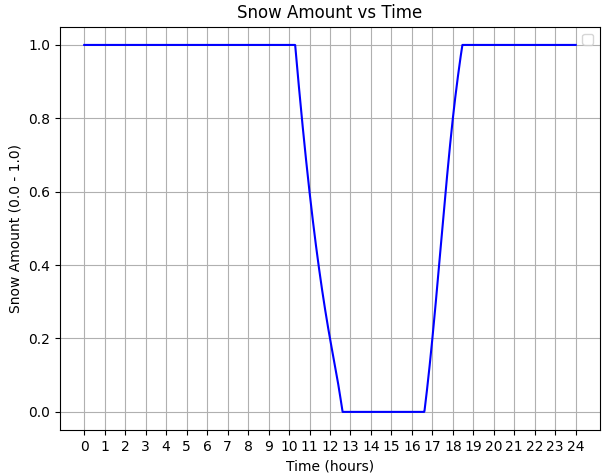
\includegraphics[width=\textwidth]{images/SnowAmount35N.png}
      \caption{Snow amount throughout the day}
      \label{fig:SnowAmount35N}
  \end{minipage}
\end{figure}

%  Environment 3: Sunlight Intensity
\subsubsection {Sunlight Intensity}
In the real world, there are multiple light sources outside, including the sun, sky, moon, stars, 
and human-made lights. In this paper, only the sunlight and sky (ambient) light are considered. 
The intensity of the skylight is a small constant value while that of the sunlight varies by 
time, ranging from 0 to 1.

Assume the light intensity of the sun is 0 (or a very small value) at night. It starts increasing 
rapidly (typically 30 minutes) before sunrise and reaches the maximum value in a short time 
(typically 1-3 hours). It remains stable until several hours before the sunset. The value 
decreases quickly in the sunset period and finally returns to 0 (or a very small value). Here is 
the mathematical formula of the light intensity.

\[
  I = e^{-\frac{\left(\frac{\pi}{2} - \theta\right)^{\frac{m}{60} + 1}}{b}}
\]

where:
\begin{itemize}
  \item \( I \) is the light intensity of the simulated sun, \( I \in (0, 1] \).
  \item \( \theta \) is the solar elevation angle in radians, which is based on the current time, 
  season (declination) and position (latitude).
  \item \( m \) is the total daylight time (in minutes) in that day, \( m \in [0, 1440) \), \( m \in \mathbb{Z} \). 
  For example, if the sunrise time is 6 AM and the sunset time is 6 PM, \( m=720 \) (12 hours)
  \item \( b \) is a bias factor adjusting the exponent decay rate, making the light intensity
  transition more realistic.
\end{itemize}

The bias \( b \) depends on multiple factors, including the altitude, latitude and time zone. To
simplify the simulation, it can be calculated by solving an equation in terms of \( m \) when 
\( I \) and \( \theta\) is given.

\[
  b = -\frac{\left(\frac{\pi}{2} - \theta\right)^{\frac{m}{60} + 1}}{\log(I)}
\]

Assume the solar light intensity is 0.1 on sunrise or sunset (i.e., \( \theta=0\)), the formula 
of the bias can be expressed as:

\[
  b = \frac{\left(\frac{\pi}{2}\right)^{\frac{m}{60} + 1}}{\log(10)}
\]

\begin{figure}[h]
  \centering
  \begin{minipage}{0.45\textwidth}
      \centering
      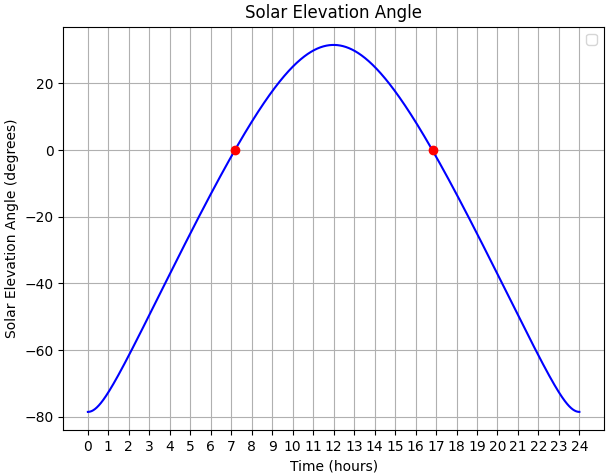
\includegraphics[width=\textwidth]{images/SolarElevetion35N.png}
      \caption{Solar elevation angle throughout the day}
      \label{fig:SolarElevetion35N}
  \end{minipage}\hfill
  \begin{minipage}{0.45\textwidth}
      \centering
      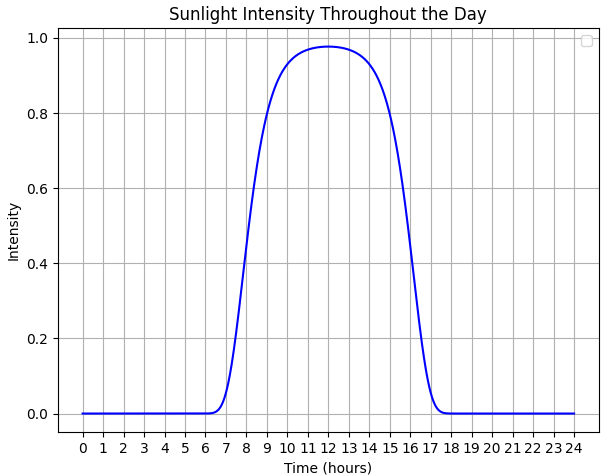
\includegraphics[width=\textwidth]{images/SunlightIntensity35N.png}
      \caption{Sunlight intensity throughout the day}
      \label{fig:SunlightIntensity35N}
  \end{minipage}
\end{figure}

% TODO: Sunlight direction

%  Environment 4: Sunlight and Sky Color
\subsubsection {Sunlight and Sky Color}
Sunlight and sky colors depend on the current time. Typically on a sunny day, the sunlight is yellow
to white for most of the day and it becomes orange during sunrise or sunset. The sky is light blue
in the day, orange during sunrise or sunset and dark purple at night. To simulate those colors, 
interpolation is also needed to make the transition process smoother. 

\[
  C_{b}=
  \left\{
    \begin{array}{ll}
      \text{night} & \theta \leq 10 \\
      \text{interpolate(night, twilight)} &  -10 \leq t < 5 \\
      \text{interpolate(twilight, day)} &  5 \leq t < 20 \\
      \text{day} & t \geq 20 \\
    \end{array} 
  \right. 
\]




\begin{figure}[h]
  \centering
  \begin{minipage}{0.45\textwidth}
      \centering
      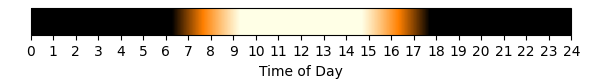
\includegraphics[width=\textwidth]{images/SunColor35N.png}
      \caption{First image caption}
      \label{fig:SunColor35N}
  \end{minipage}\hfill
  \begin{minipage}{0.45\textwidth}
      \centering
      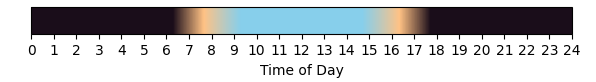
\includegraphics[width=\textwidth]{images/SkyColor35N.png}
      \caption{Second image caption}
      \label{fig:SkyColor35N}
  \end{minipage}
\end{figure}


\section{Experiments and Results}
\subsection {Pure Snow Effect}
The following figure group is the rendering effect with full snow, half snow, and no snow respectively.
The dynamic environment system is disabled and the light source is always right above the object with
the maximum intensity and white color. Those three sub-figures illustrate the effect on both declination 
(the head and book of the statue) and occlusion (the feet area of it), as well as the color blending
mentioned above.

\begin{figure}[h]
  \centering
  \subfloat[Snow Amount = 0.0]{
    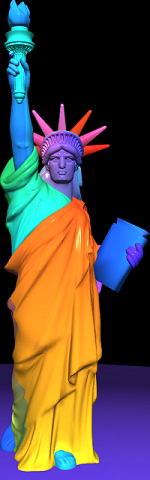
\includegraphics[width=0.30\textwidth]{images/AllTimeNaNNoSnow.png}
    \label{fig:AllTimeNaNNoSnow}
  }\hfill
  \subfloat[Snow Amount = 0.5]{
    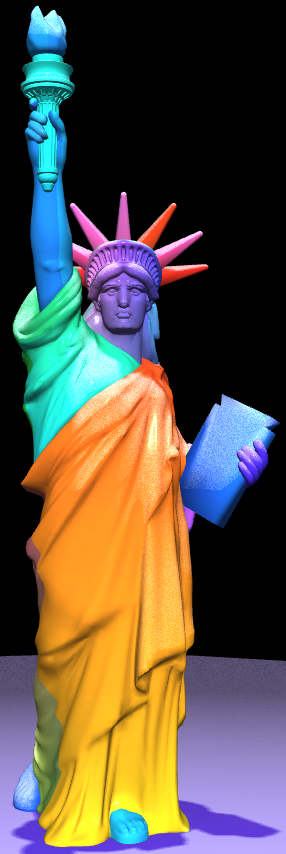
\includegraphics[width=0.30\textwidth]{images/AllTimeNaNHalfSnow.png}
    \label{fig:AllTimeNaNHalfSnow}
  }\hfill
  \subfloat[Snow Amount = 1.0]{
    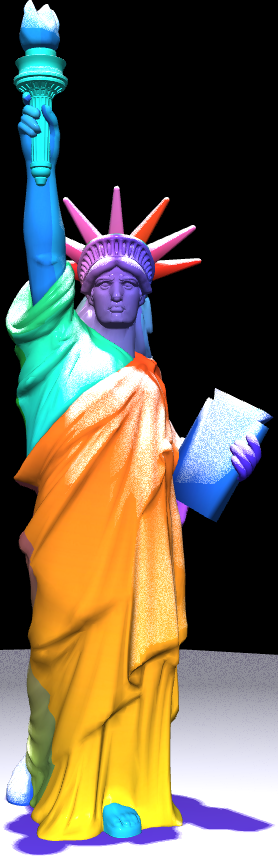
\includegraphics[width=0.30\textwidth]{images/AllTimeNaNFullSnow.png}
    \label{fig:AllTimeNaNFullSnow}
  }
  \caption{Object covered by different amounts of snow}
  \label{fig:9}
\end{figure}

\subsection {Snow Effect with Dynamic Daylight Simulation}
\label{headings}
The following figure group is the rendering effect at different times with the location mentioned above.
The snow is fully covered throughout the night (a) with only ambient color. In the morning, the sunlight
intensity increases with an orange color, causing the orange-to-yellow snow color (b). When the clock hits 
10 AM, it is bright enough but the snow coverage is still 100 \% as the temperature is still below 
\(0^\circ\mathrm{C}\) (c). The snow starts melting at 11 AM (d). The weather is warmest at 2 PM, as a result,
there is no snow on the scene (e). During the sunset period, the snow emerges back due to the low temperature (f).

\begin{figure}[h]
  \centering
  \subfloat[Time = 12 AM]{
    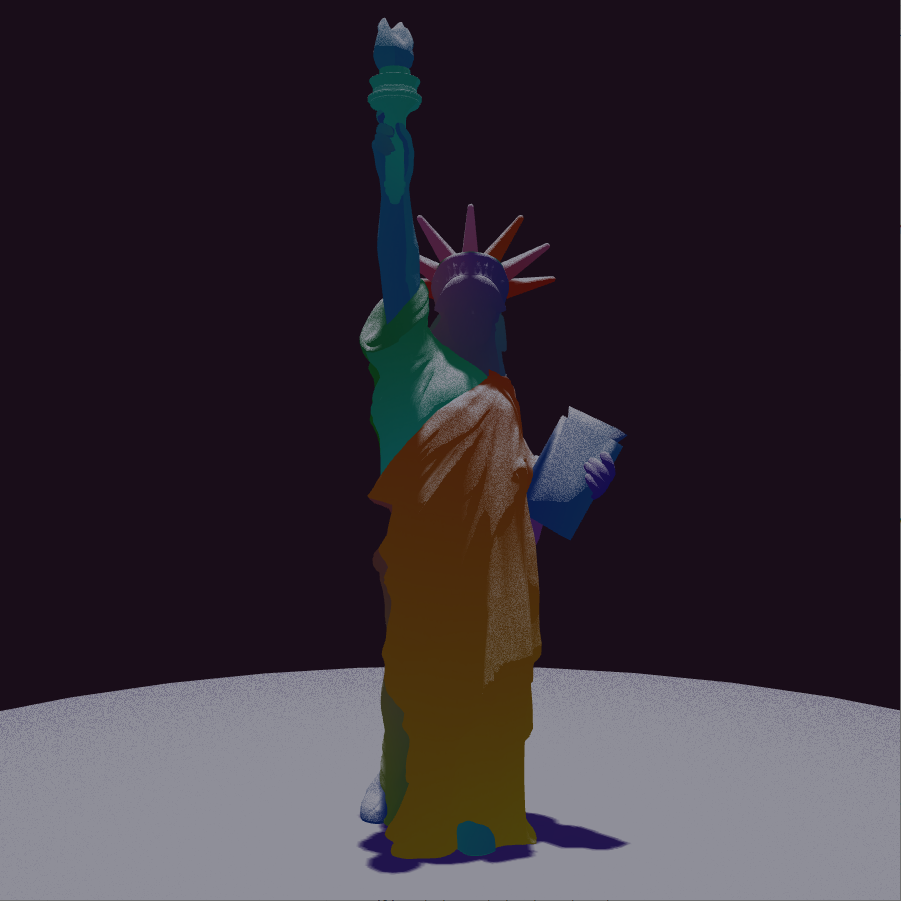
\includegraphics[width=0.3\textwidth]{images/AllT0000L35N.png}
    \label{fig:AllT0000L35N}
  }\hfill
  \subfloat[Time = 8 AM]{
    
\includegraphics[width=0.3\textwidth]{images/AllT0800L35N.png}
    \label{fig:AllT0800L35N}
  }\hfill
  \subfloat[Time = 10 AM]{
    
\includegraphics[width=0.3\textwidth]{images/AllT1000L35N.png}
    \label{fig:AllT1000L35N}
  }

  \subfloat[Time = 11 AM]{
    
\includegraphics[width=0.3\textwidth]{images/AllT1100L35N.png}
    \label{fig:AllT1100L35N}
  }\hfill
  \subfloat[Time = 2 PM]{
    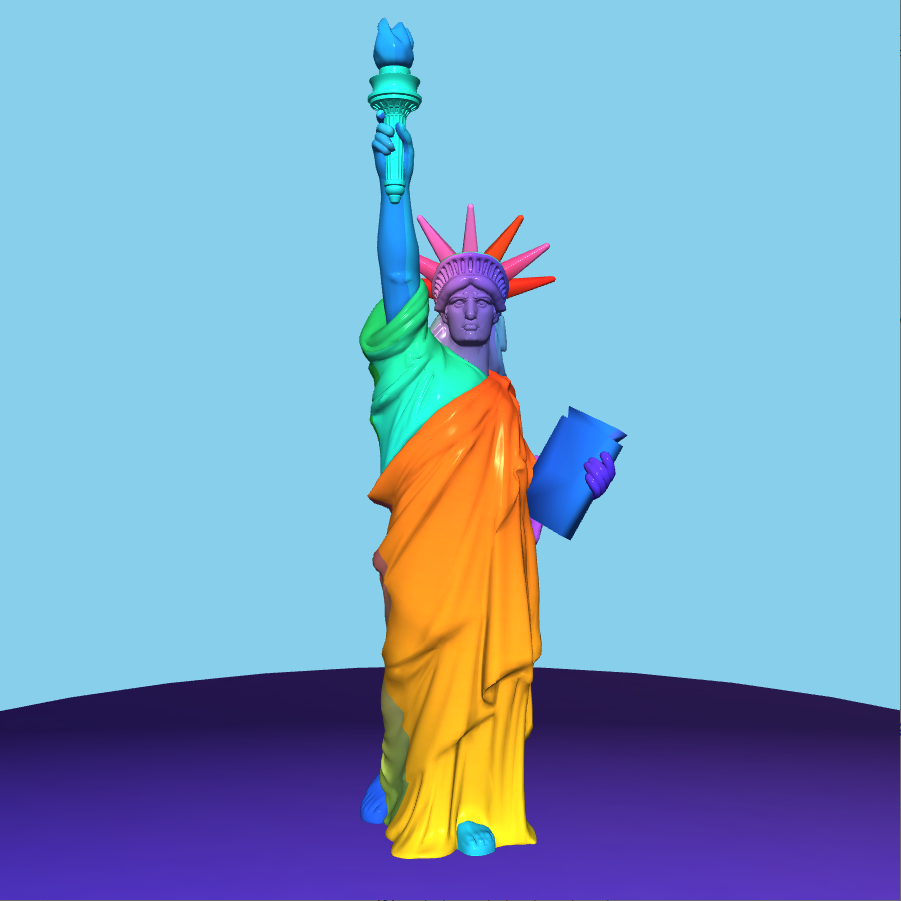
\includegraphics[width=0.3\textwidth]{images/AllT1400L35N.png}
    \label{fig:AllT1400L35N}
  }\hfill
  \subfloat[Time = 5 PM]{
    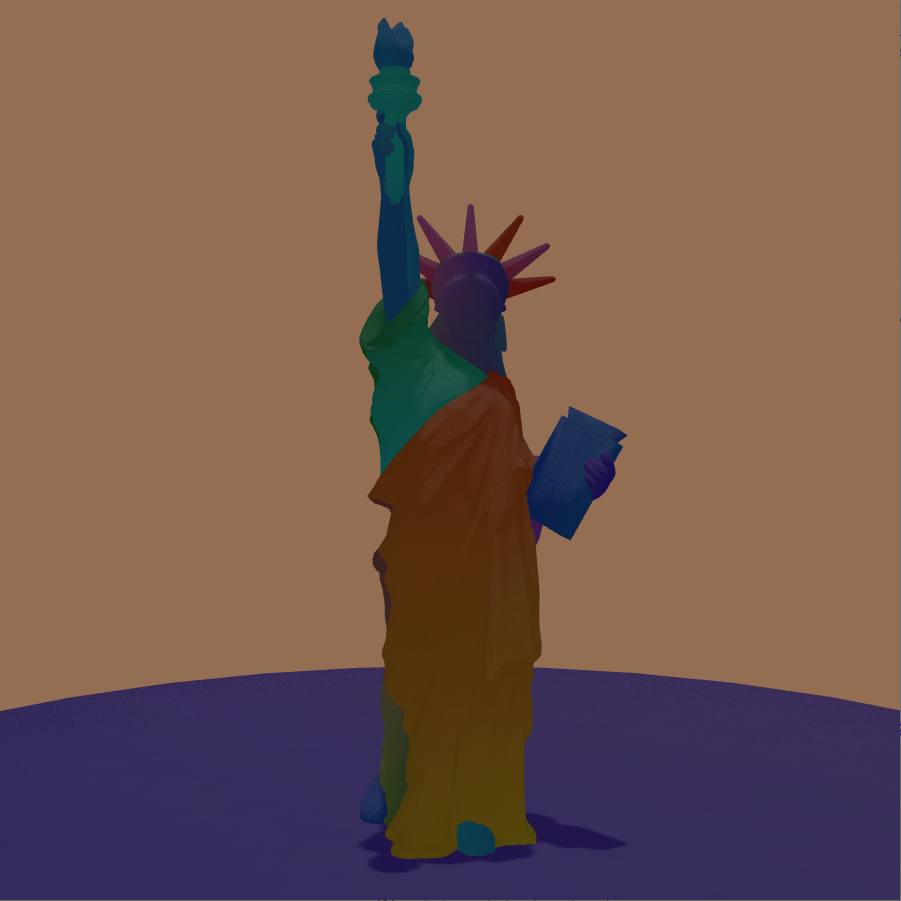
\includegraphics[width=0.3\textwidth]{images/AllT1700L35N.png}
    \label{fig:AllT1700L35N}
  }

  \caption{The rendered scene in different time}
  \label{fig:mainfigure}
\end{figure}

First-level headings should be in 12-point type.

\begin{figure}[h]
  \centering
  \subfloat[Time = 12 AM]{
    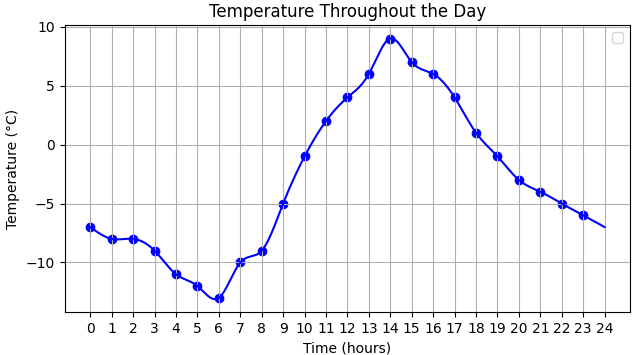
\includegraphics[width=0.3\textwidth]{images/Temperature60N.png}
    \label{fig:image1}
  }\hfill
  \subfloat[Time = 8 AM]{
    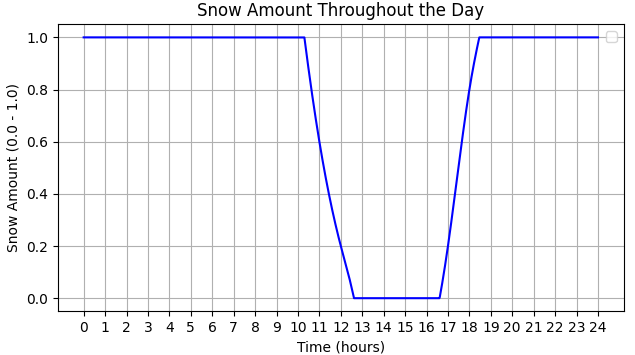
\includegraphics[width=0.3\textwidth]{images/SnowAmount60N.png}
    \label{fig:image2}
  }\hfill
  \subfloat[Time = 10 AM]{
    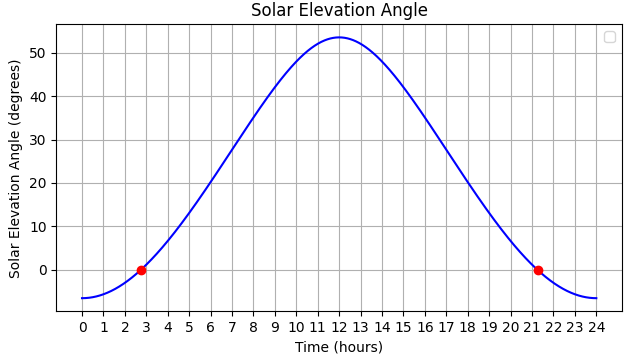
\includegraphics[width=0.3\textwidth]{images/SolarElevetion60N.png}
    \label{fig:image3}
  }

  \subfloat[Time = 11 AM]{
    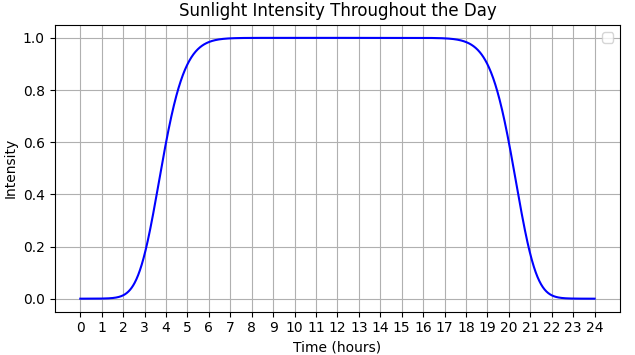
\includegraphics[width=0.3\textwidth]{images/SunlightIntensity60N.png}
    \label{fig:image4}
  }\hfill
  \subfloat[Time = 2 PM]{
    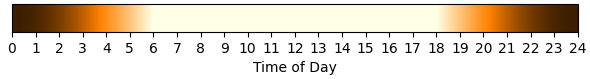
\includegraphics[width=0.3\textwidth]{images/SunColor60N.png}
    \label{fig:image5}
  }\hfill
  \subfloat[Time = 5 PM]{
    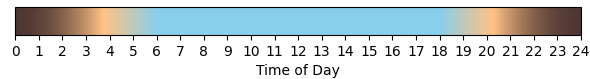
\includegraphics[width=0.3\textwidth]{images/SkyColor60N.png}
    \label{fig:image6}
  }

  \caption{The rendered scene in different time}
  \label{fig:mainfigure}
\end{figure}










\section{Discussions and Conclusion}


Please prepare submission files with paper size ``US Letter,'' and not, for
example, ``A4.''


Fonts were the main cause of problems in the past years. Your PDF file must only
contain Type 1 or Embedded TrueType fonts. Here are a few instructions to
achieve this.


\section*{References}

{
\small


[1] Alexander, J.A.\ \& Mozer, M.C.\ (1995) Template-based algorithms for
connectionist rule extraction. In G.\ Tesauro, D.S.\ Touretzky and T.K.\ Leen
(eds.), {\it Advances in Neural Information Processing Systems 7},
pp.\ 609--616. Cambridge, MA: MIT Press.


[2] Bower, J.M.\ \& Beeman, D.\ (1995) {\it The Book of GENESIS: Exploring
  Realistic Neural Models with the GEneral NEural SImulation System.}  New York:
TELOS/Springer--Verlag.


[3] Hasselmo, M.E., Schnell, E.\ \& Barkai, E.\ (1995) Dynamics of learning and
recall at excitatory recurrent synapses and cholinergic modulation in rat
hippocampal region CA3. {\it Journal of Neuroscience} {\bf 15}(7):5249-5262.
}
\section*{Additional Experiment Results}

\section*{Confidential Peer Review} 

The percentage, who did what, ratio weights. 






\end{document}